\documentclass[twoside,a4paper,12pt]{article}
\usepackage[applemac]{inputenc}
\usepackage{wrapfig}
\usepackage{graphicx}
\usepackage{graphics}
%\usepackage{subfig}
%\usepackage{inputenc}
\usepackage{amsmath}
\usepackage{amsfonts}
\usepackage{amssymb}
\usepackage[singlelinecheck=false]{caption}
\usepackage{array}
\usepackage{multirow}
\usepackage{setspace}
\usepackage{hyperref}
\usepackage{verbatim}
\usepackage[clearempty]{titlesec}
\usepackage{epstopdf}
\usepackage{lineno}
\usepackage{textcomp}
\usepackage{nicefrac}
\usepackage{xspace}
%\usepackage{autoref}
\usepackage[small, bf, hang, raggedright]{subfigure}

\usepackage[english]{babel} 

\onehalfspacing
\usepackage[left=2.9cm,right=2.9cm,top=3cm,bottom=4.5cm]{geometry}
\newcommand\leerseite{\newpage\thispagestyle{empty}\hspace{1cm}\newpage}

\newcommand{\subfigureautorefname}{\figurename}

\newcommand\piminus{\(\mathrm{\pi^-}\)}
\newcommand\muminus{\(\mathrm{\mu^-}\)}
\newcommand\eminus{\(\mathrm{e^-}\)}
\newcommand\eplus{\(\mathrm{e^+}\)}
\newcommand\geant{\textsc{Geant\,4}\xspace}

\begin{document}\selectlanguage{english}




\section*{Answers to Daniel's comments from 01.03.2016}
Hi Daniel,
thank you very much for your thorough reading and insightful comments!
Please find my answers between your quotes below:

\begin{quote}\texttt{Plots should probably mention "ScECAL+AHCAL+TCMT" in addition to "CALICE preliminary".}\end{quote}
I agree. I changed all plots accordingly (and cleaned up some of the legends in the process). 

\begin{quote}\texttt{l42: references should appear in order. (i.e. [1,2] not [7,12]).}\end{quote}
done.

\begin{quote}\texttt{l45: the thickness of the ECAL in terms of lambda is also of interest, and should be quoted here.}\end{quote}
done.

\begin{quote}\texttt{l85: "light yield" should be two words.}\end{quote}
done.

\begin{quote}\texttt{l108: "channel--wise"}\end{quote}
done

\begin{quote}\texttt{Fig1 caption: Given the non-Gaussian distribution, I guess that "\\sigma" is actually the RMS of the distribution? 
In which case RMS\_{data} would be better.}\end{quote}
You are right, done.

\begin{quote}\texttt{L121: I have difficulty imagining how a wrong material description would significantly suppress high energy hits...}\end{quote}
I tried to explain this in lines 132-140. A wrong material description can lead to a too small Moliere radius, leading to narrower showers, leading to harder hit energy spectra. 

\begin{quote}\texttt{Fig3: As we already discussed when we met in person, the transverse profile of EM showers could be affected by layer-to-layer
misalignments. How well were these controlled?
A layer-by-layer profile, in which hit positions are compared to the cluster centre in that layer, would factor out this
effect.}\end{quote}
This is a very good idea, we did not think of that before! Doing the plot as you propose it, plotting the ``mean radius'' vs. layer number is possibly very dependent on the noise overlay and might show some artifacts due to the limited number of noise events repeatedly overlaid over the MC events, so instead I did the following:   
I redid the transverse shower profile plot, but now using the center of gravity extracted for each layer individually instead of the whole shower as the reference position. If layer misalignment is the cause for the data/MC discrepancy in fig. 3(b) of the draft, the new plots should show a significant improvement. The new plot is shown in \autoref{fig:transverse_cog}. The discrepancy between data and simulation does not change in shape or magnitude to the plot in the draft. I will keep the previous plot in the note, as it is easier to understand what is done.

\begin{figure}[htbp]
\begin{center}
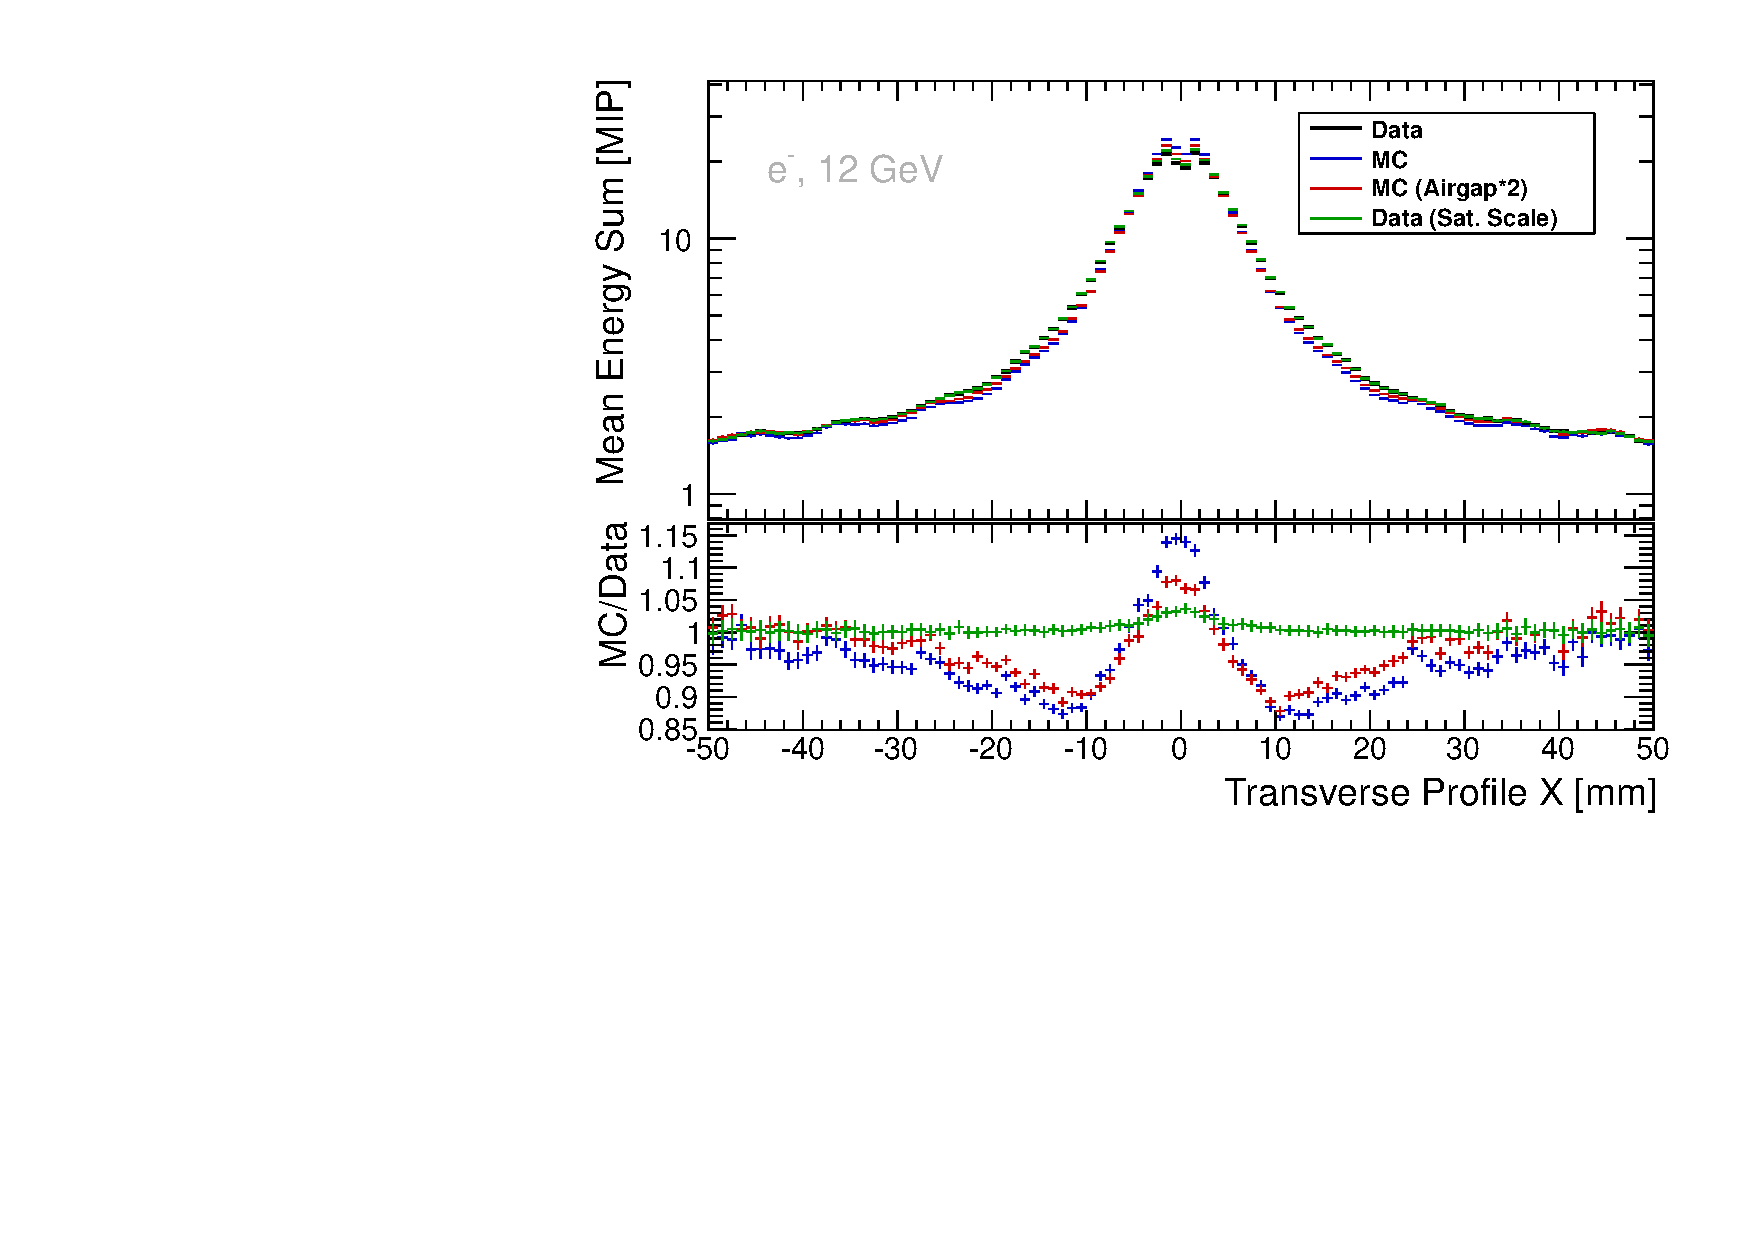
\includegraphics[width=0.8\textwidth,page=1]{out_profileRadial_LayerCoG_560294_12GeV}
\caption{Transverse electron shower profile in the ScECAL. Instead of using the full shower center of gravity as the shower axis, the center of gravity calculated for each layer individually is used.}
\label{fig:transverse_cog}
\end{center}
\end{figure}

\begin{quote}\texttt{L212: how did you estimate 10e-2? If I look at the shoulder above 45 GeV in fig 5(a), which seems to be to most 
obvious contribution not in the MC, it looks rather smaller than 1\% integrating a log-scale distribution by eye...)}\end{quote}
 

\begin{quote}\texttt{L232: weighted down -> de-weighted}\end{quote}
done.

\begin{quote}\texttt{L260: the e/pi ratio is in general not necessarily <1 in general. 
Either make this sentence more specific to refer only to the calorimeters studied here, or soften the statement.}\end{quote}
Done. Changed to: ``For most calorimeters, the measured response generated by a hadron shower [...]''


\begin{quote}\texttt{Fig6 caption, last sentence: I suppose that the uncertainties you refer to are the statistical ones?
If so, it's better to write it.}\end{quote}
You are right, done.

\begin{quote}\texttt{L282: you introduce rho, but as far as I can understand you do not use this energy density (L291).}\end{quote}
This is true. This paragraph discusses the general concept, while the next paragraph explains the actual implementation. I altered the text slightly to make this more clear  (ll. 297-310 in the updated draft).

\begin{quote}\texttt{L284: how do you decide the binning? Are the results you get independent of the chosen binning?}\end{quote}
The binning was chosen rather arbitrarily: The first bin was chosen from the hit energy threshold 0.5MIP up to 2MIP to mostly accomodate single particle hits (mind that the mean deposition of one minimum-ionising particles is ~1.4 MIP. Also the hit energy distribution is falling rather steeply at low hit energies, see \autoref{fig:hitenergies_inner_outer}). The second bin 2MIP--4MIP is chosen to have mostly two-particle hits (for the same reasons as the first bin). The other bins are made to be equidistant on a log-X scale up to the chosen maximum point of 100MIP for the ScECAL and 50MIP for the AHCAL. The number of bins was chosen to be significantly more than the SDHCAL, but not too many to keep the number of optimisation parameters reasonable. 

The results do not depend on the exact bin boundaries or number of bins. Coralie's updated note (results will be shown at the upcoming CALICE meeting I believe) will show that 3 bins work only slightly worse than 8--10 bins. 

Added sentence ``The obtained resolutions do not critically depend on the number bins or exact bin boundaries'' to clarify (l. 311 in updated draft).

\begin{quote}\texttt{L291: I think that the fact of using the hit energy, rather than the energy density, means you are in effect
de-weighting the outer cells, which also tend to be the cells with a smaller energy (and less EM content).
I wonder if doing this limits the applicability of your results to a uniformly tiled HCAL?
If the improvement you get is only limited, might it be simpler/cleaner to use the energy density?}\end{quote}
Measuring a deposition of around 1MIP is in the very most cases exactly one traversing particle (disregarding downward fluctuations from the Landau and photon statistics). No single particle can deposit less than that energy (apart from very low energy particles that get stuck and deposit all their remaining kinetic energy in a tile). So for depositions around 1 MIP, dividing by the tile area for density does not really make sense, as we know the deposition is not distributed over the tile surface but most likely came from a single particle. Most of all hits are around the single MIP level anyway, even more so in the outer parts of the AHCAL, as shown in \autoref{fig:hitenergies_inner_outer} (please excuse the ugly quick and dirty plot).
\begin{figure}[htbp]
\begin{center}
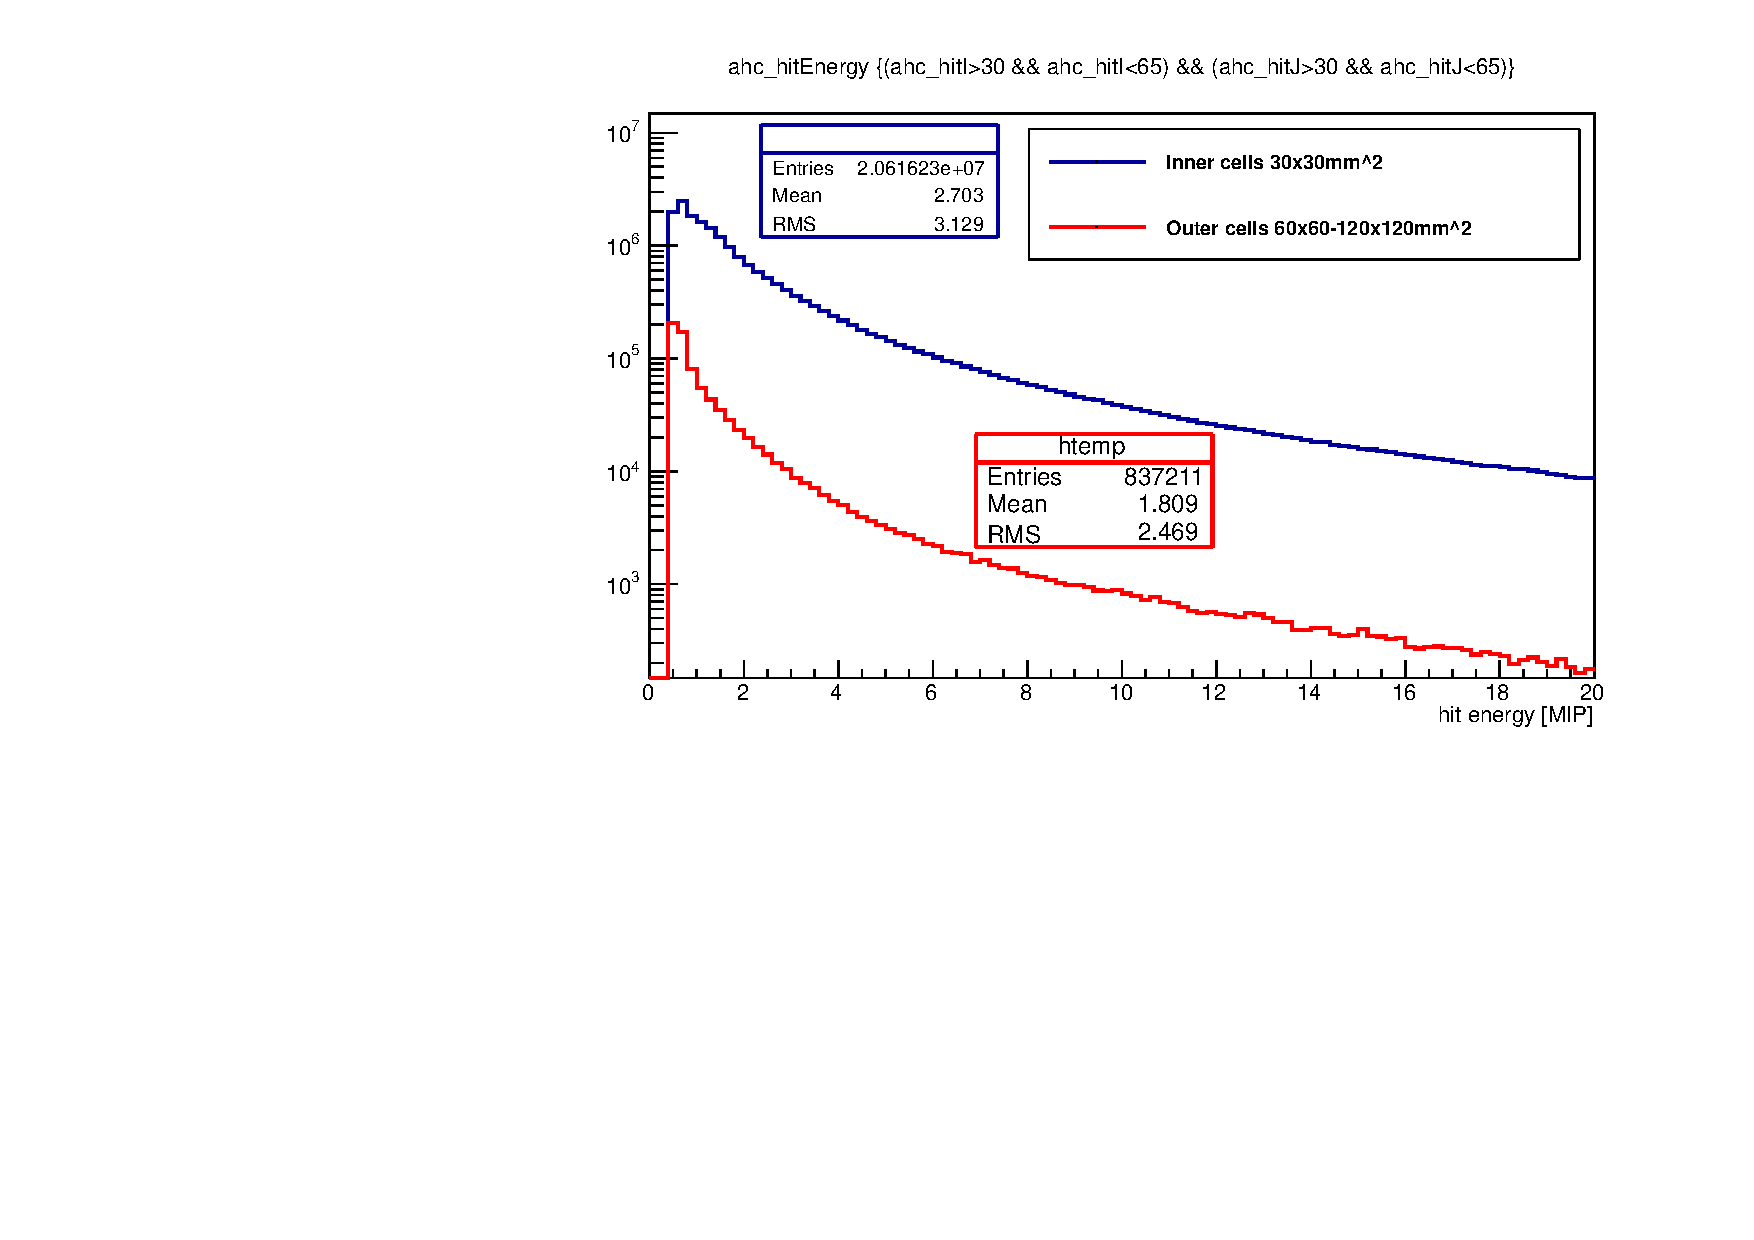
\includegraphics[width=0.8\textwidth,page=1]{hitenergy_AHCAL_inner_vs_outer_cells_560474_MC}
\caption{AHCAL Hit energy distribution of the central, finely segmented core of 30*30mm\textsuperscript{2} tiles and the outer, coarser rings of 60*60 to 120*120\textsuperscript{2} tiles.}
\label{fig:hitenergies_inner_outer}
\end{center}
\end{figure}
 When using the true measured deposition density instead of the hit energy, most energy depositions of the larger AHCAL cells will fall into the first two hit energy bins (0.5-2MIP), which is also not really what we want to do. Ideally one would have separate software compensation weights for each tile size. In practice there is not enough statistics in these cells to do that, and the number of parameters and computation time in optimisation would increase by an unreasonable amount.

The applicability of this procedure to uniformly tiled calorimeters is shown in Coralie's currently updated CAN-049.
  
\begin{quote}\texttt{L294: "first two bins" -> "two lowest energy bins"}\end{quote}
done.

\begin{quote}\texttt{L312: from the plot, it looks like rather less than "half".}\end{quote}
True, and it depends on beam energy. The fraction of hits identified as primary track hits in the first two bins is actually 50\% at 4GeV but only 20\% at 32GeV. Sentence adjusted to ``around one quarter'' (l. 330 in the updated draft).

\begin{quote}\texttt{L315: "most selected events" -> can you be more quantitative? 
Consider including a plot of the FHI layer for illustration.}\end{quote}
70\% of selected events have reconstructed FHI layer in the ScECAL. The plot of reconstructed FHI layer in data and MC was removed due to length of the paper. I have put the plot back into the note (into the event selection section, l.196) and reference it again when talking about of fraction of hits on tracks in line 333 of the updated draft.

\begin{quote}\texttt{Fig8: The y-axis labels both refer to the same quantity, I think: please unify the labels.}\end{quote}
Done. Fig.11 also has the same y-axis and showed yet another title for it. It's all labelled ``Hit Energy Bin Weight'' now. 

\begin{quote}\texttt{It's not immediately obvious why the first two bins of (c) and (d) have a slope.}\end{quote}
added ``the hit energy dependent weights of the first two bins correspond to a $\nicefrac{1}{E}$ dependence and thus a counting of hits in these bins.'' in plot caption on p.18.
 
\begin{quote}\texttt{Some of the colors in (a) and (b) are impossible to distinguish.}\end{quote}
Finding 8 colors that are easily distinguished on screen, print and projector presentation is difficult. The plot would typically be shown accompanied by (b)/(c), helping to explain what is going on. I could produce a version of the plot with less bins (showing bins 1, 4, 8 for example) for presentations. Do you think this would help? 

\begin{quote}\texttt{(a) shows a large jump between bins 2 and 3. 
Might it be better to use finer binning in this region to smooth the behaviour somewhat?
Or is this just an effect of going from hit counting to energy counting?}\end{quote}
This is mostly an effect from the counting and misguiding the eye from the sloped bins. In a previous, separate study I saw no difference in resolution between 8 bins and 40 bins. However I could change the reconstruction to only count hits in the first bin. What do you think?

\begin{quote}\texttt{L400: just out of interest, is the length of showers well simulated in the W-AHCAL with these physics lists?
This could help point the finger at tungsten, or elsewhere.}\end{quote}
Eva's paper (``Shower development of particles with momenta from 15 GeV to 150 GeV in the CALICE scintillator-tungsten hadronic calorimeter'') does show similar data/MC ratios and spread in MCs for the W-AHCAL shower profile from FHI, as I have for the scecal in fig.13(a) (fig.14(a) in the new draft). Compared to my plot, Eva's plot looks a bit better by eye, but I think my plot just shows less range in the X-axis.

In addition to the changes triggered by your comments, I fixed a mistake in table A2 (containment cut of the electron selection).

I have uploaded the updated version of the note including the two animations to INDICO.

Cheers,
Oskar


\end{document}
